\documentclass[border=4pt]{standalone}
% Preámbulo común de las figuras. Cada figura es un documento standalone
% que se compila a SVG con scripts/build_figures.sh
\usepackage[utf8]{inputenc}
\usepackage{amsmath}
\usepackage{tikz}
\usepackage[american, siunitx]{circuitikz}
\usetikzlibrary{arrows.meta,calc,decorations.pathmorphing,patterns}
\tikzset{
  >={Stealth[length=2.2mm]},
  eje/.style={->, thin},
  hilo/.style={thick},
}
% Paleta común: tonos medios legibles sobre fondo claro
\definecolor{azul}{RGB}{31,94,168}
\definecolor{rojo}{RGB}{192,57,43}
\definecolor{verde}{RGB}{39,128,73}
\definecolor{naranja}{RGB}{211,120,30}
\definecolor{morado}{RGB}{125,60,152}

\begin{document}
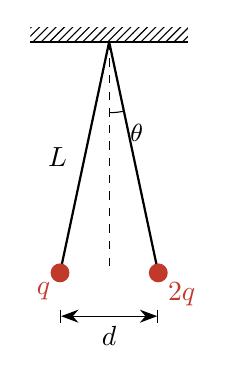
\begin{tikzpicture}[scale=1.0]
  \fill[pattern=north east lines] (-1.0,0) rectangle (1.0,0.18);
  \draw[thick] (-1.0,0) -- (1.0,0);
  \draw[dashed] (0,0) -- (0,-2.934);
  \draw[hilo] (0,0) -- (-0.624,-2.934);
  \draw[hilo] (0,0) -- (0.624,-2.934);
  \fill[rojo] (-0.624,-2.934) circle (0.12) node[below left]{$q$};
  \fill[rojo] (0.624,-2.934) circle (0.12) node[below right]{$2q$};
  \draw (0,-0.9) arc[start angle=-90, end angle=-78, radius=0.9];
  \node[font=\small] at (0.35,-1.15) {$\theta$};
  \node[left] at (-0.412,-1.467) {$L$};
  \draw[|<->|] (-0.624,-3.484) -- node[below]{$d$} (0.624,-3.484);
\end{tikzpicture}
\end{document}
